\section{Resultados y discusión}
Con el objetivo de determinar la frecuencia de corte $f_0$ de un circuito RC y la frecuencia de resonancia $f_r$ de un circuito RLC, se estudió la respuesta de ambos circuitos para distintas frecuencias como señal de entrada, haciendo uso del lenguaje de programación $Python$ \cite{github}.

\subsection{Circuito RC}

Para el circuito RC, según se mida en configuración PA o PB, se muestra el diagrama de bode correspondiente en la \autoref{fig:rectasRC}. Se graficó el módulo de $H$ en decibeles y la fase $\phi$ en función de $\omega$, donde $f_0$ se determinó a partir del punto de intersección entre dos rectas, ajustadas con pendiente libre (indicadas en violeta) y con pendiente nula (indicadas en naranja).

\begin{figure}[H]
    \centering
    
\includegraphics[width=1\linewidth]{gráficos/bode_completo_rc.png}
    \caption{Diagramas de Bode para el filtro PA (izq.) y para el filtro PB (der.). En rosa se indica el ajuste realizado para la fase, junto al
     \(\tau\) obtenido. En naranja, se presentan los datos ajustados por la recta con pendiente $m$ = 0. En violeta, los datos ajustados por la recta con pendiente $m$ libre. El punto de intersección entre las dos rectas se indica en negro, el cual se asigna a la  frecuencia de corte $\omega_0$.}
    \label{fig:rectasRC}
\end{figure}

Para el filtro PA se obtuvo $f_0$ = \SI{1851(176)}{\hertz}, mientras que para el filtro PB, la frecuencia obtenida fue $f_0$ = \SI{1535(207)}{\hertz}. Finalmente, se calculó el promedio ponderado utilizando ambas magnitudes, obteniendo como frecuencia de corte $f_0$ = \SI{1718(134)}{\hertz}. Además, con el objetivo de verificar que tan adecuada resulta la determinación de $f_0$ utilizando el método de intersección de rectas, se ajustó una función arcotangente según la relación del ángulo de desfasaje para el filtro PA \eqref{eq:3} y para el filtro PB \eqref{eq:4}, dejando a $\tau$ como parámetro libre. Las determinaciones de $\tau$ fueron congruentes entre sí, obteniendo para ambos filtros el valor de \SI{88 (3)}{\micro\second}. Se calculó el promedio ponderado de los resultados, dando $\tau$ = \SI{88 (2)}{\micro\second}, lo cual conduce a una frecuencia de corte $f_0 = \frac{1}{2\pi\tau}$ = \SI{1814(45)}{\hertz}. La $f_0$ obtenida resulta congruente con la determinada a través del método de intersección de rectas, respaldando la validez del método para la caracterización de sistemas de primer orden. Finalmente, se calculó el promedio ponderado de ambos métodos, obteniendo $f_0$ = \SI{1804(43)}{\hertz}, compatible con la frecuencia de referencia calculada a partir de los valores nominales de los componentes de $f_{0_{ref}}$ = \SI{1592(178)}{\hertz}.

Se realizaron los diagramas de Nyquist para el circuito RC en ambas configuraciones, como filtro PA y filtro PB, presentados en la \autoref{fig:nyquist_RC}. En naranja, se observan los datos obtenidos para el filtro PA, mientras que en violeta, los datos obtenidos para el filtro PB. Ambas series de datos se presentan superpuestas con las curvas teóricas dadas por las ecuaciones \eqref{PA} y \eqref{PB}, junto a sus fases asociadas \eqref{eq:3} y \eqref{eq:4}, las cuales resultan compatibles con los diagramas de Nyquist esperados para cada configuración.

\begin{figure}[H]
    \centering
    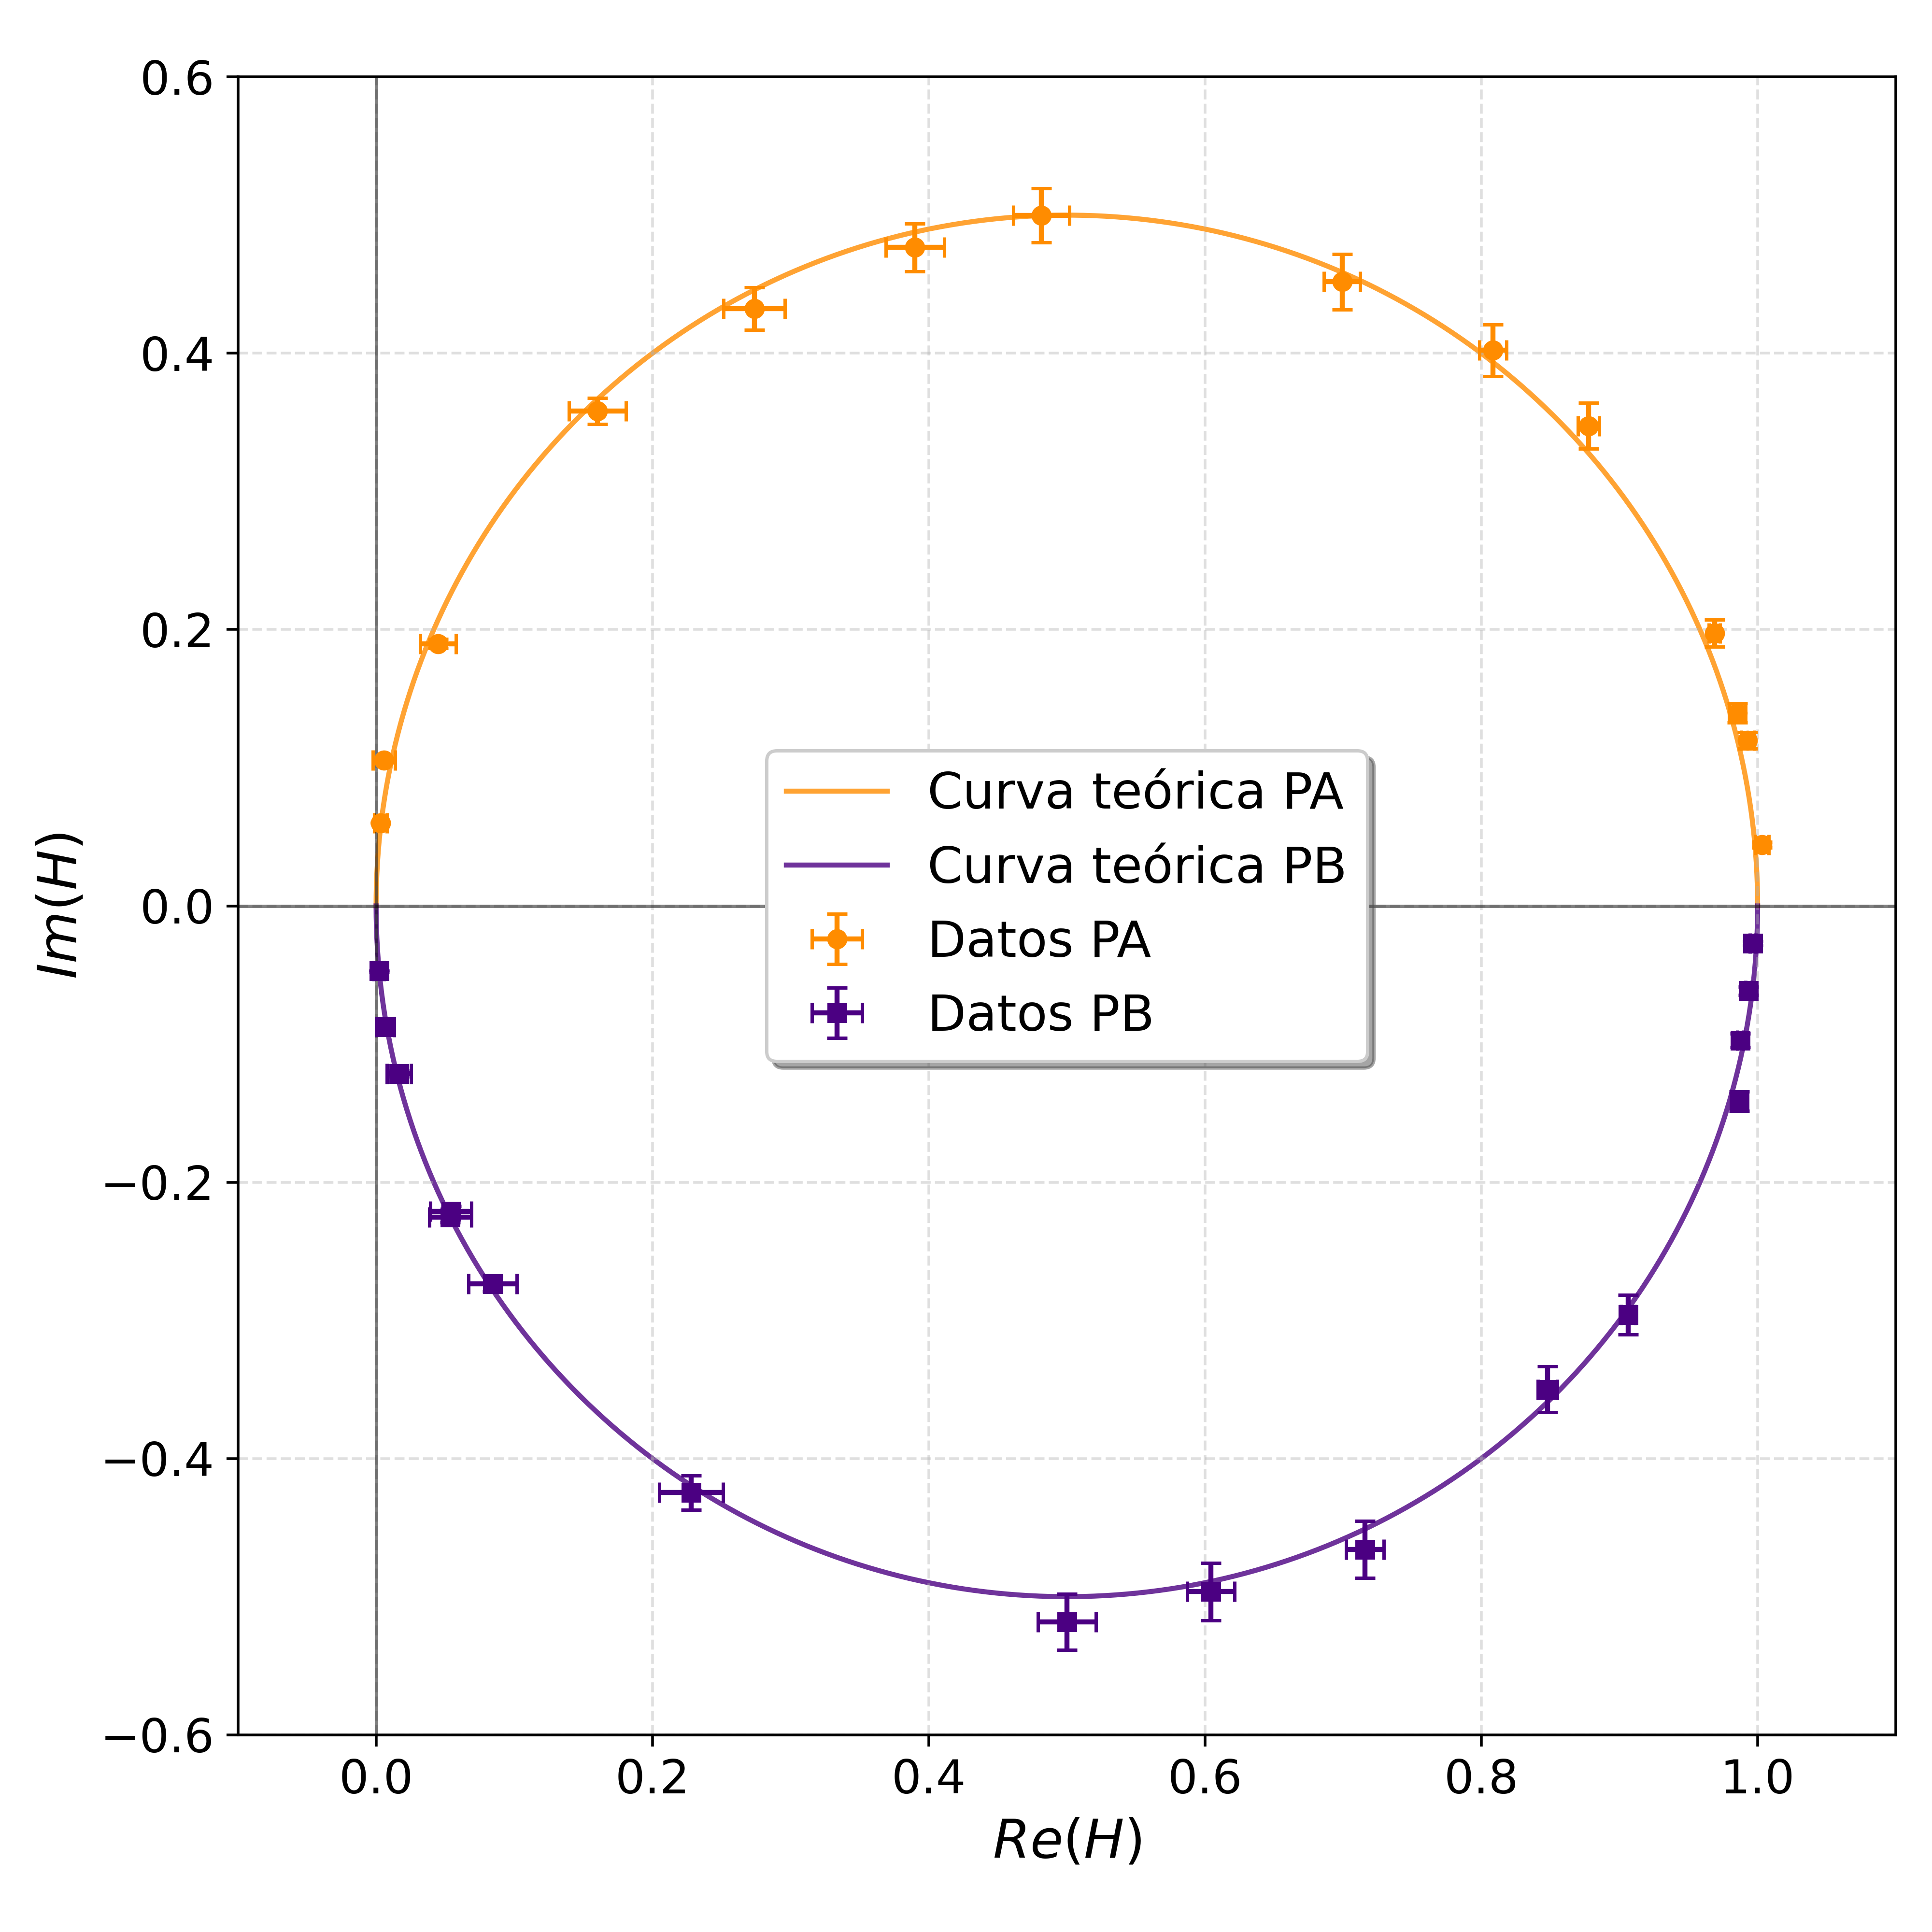
\includegraphics[width=0.5\linewidth]{gráficos/nyquist_RC_con_teoria.png}
    \caption{Diagramas de Nyquist realizados para los filtros PA y PB. En naranja, se indican los datos obtenidos con el filtro PA, mientras que en violeta se muestran los datos obtenidos con el filtro PB, ambos con su curva teórica correspondiente.}
    \label{fig:nyquist_RC}
\end{figure}

\subsubsection{Circuito RLC}
Para el circuito RLC, se obtuvo la frecuencia de resonancia $f_r$ a partir del ajuste de la expresion \eqref{eq:moduloRLC} y \eqref{eq:desfasajeRLC}. Con la primera expresión se realizaron dos ajustes, dejando el parámetro $\tau$ libre, caracterizado como un $\tau_{ef}$ efectivo del sistema, y fijando $\tau_{exp}$ al obtenido experimentalmente por el promedio ponderado del los ajustes del circuito RC. Con la segunda expresión se dejó como parámetro libre el \(\tau\) deseado. Dichos ajustes se presentan superpuestos en la \autoref{fig:tau_RLC}. Los resultados utilizando tau como parámetro libre resultaron congruentes entre sí, por lo que se obtuvo un promedio ponderado de \(f_r= 3318(19)\) \SI{}{\hertz}. 
\begin{figure}[H]
    \centering
    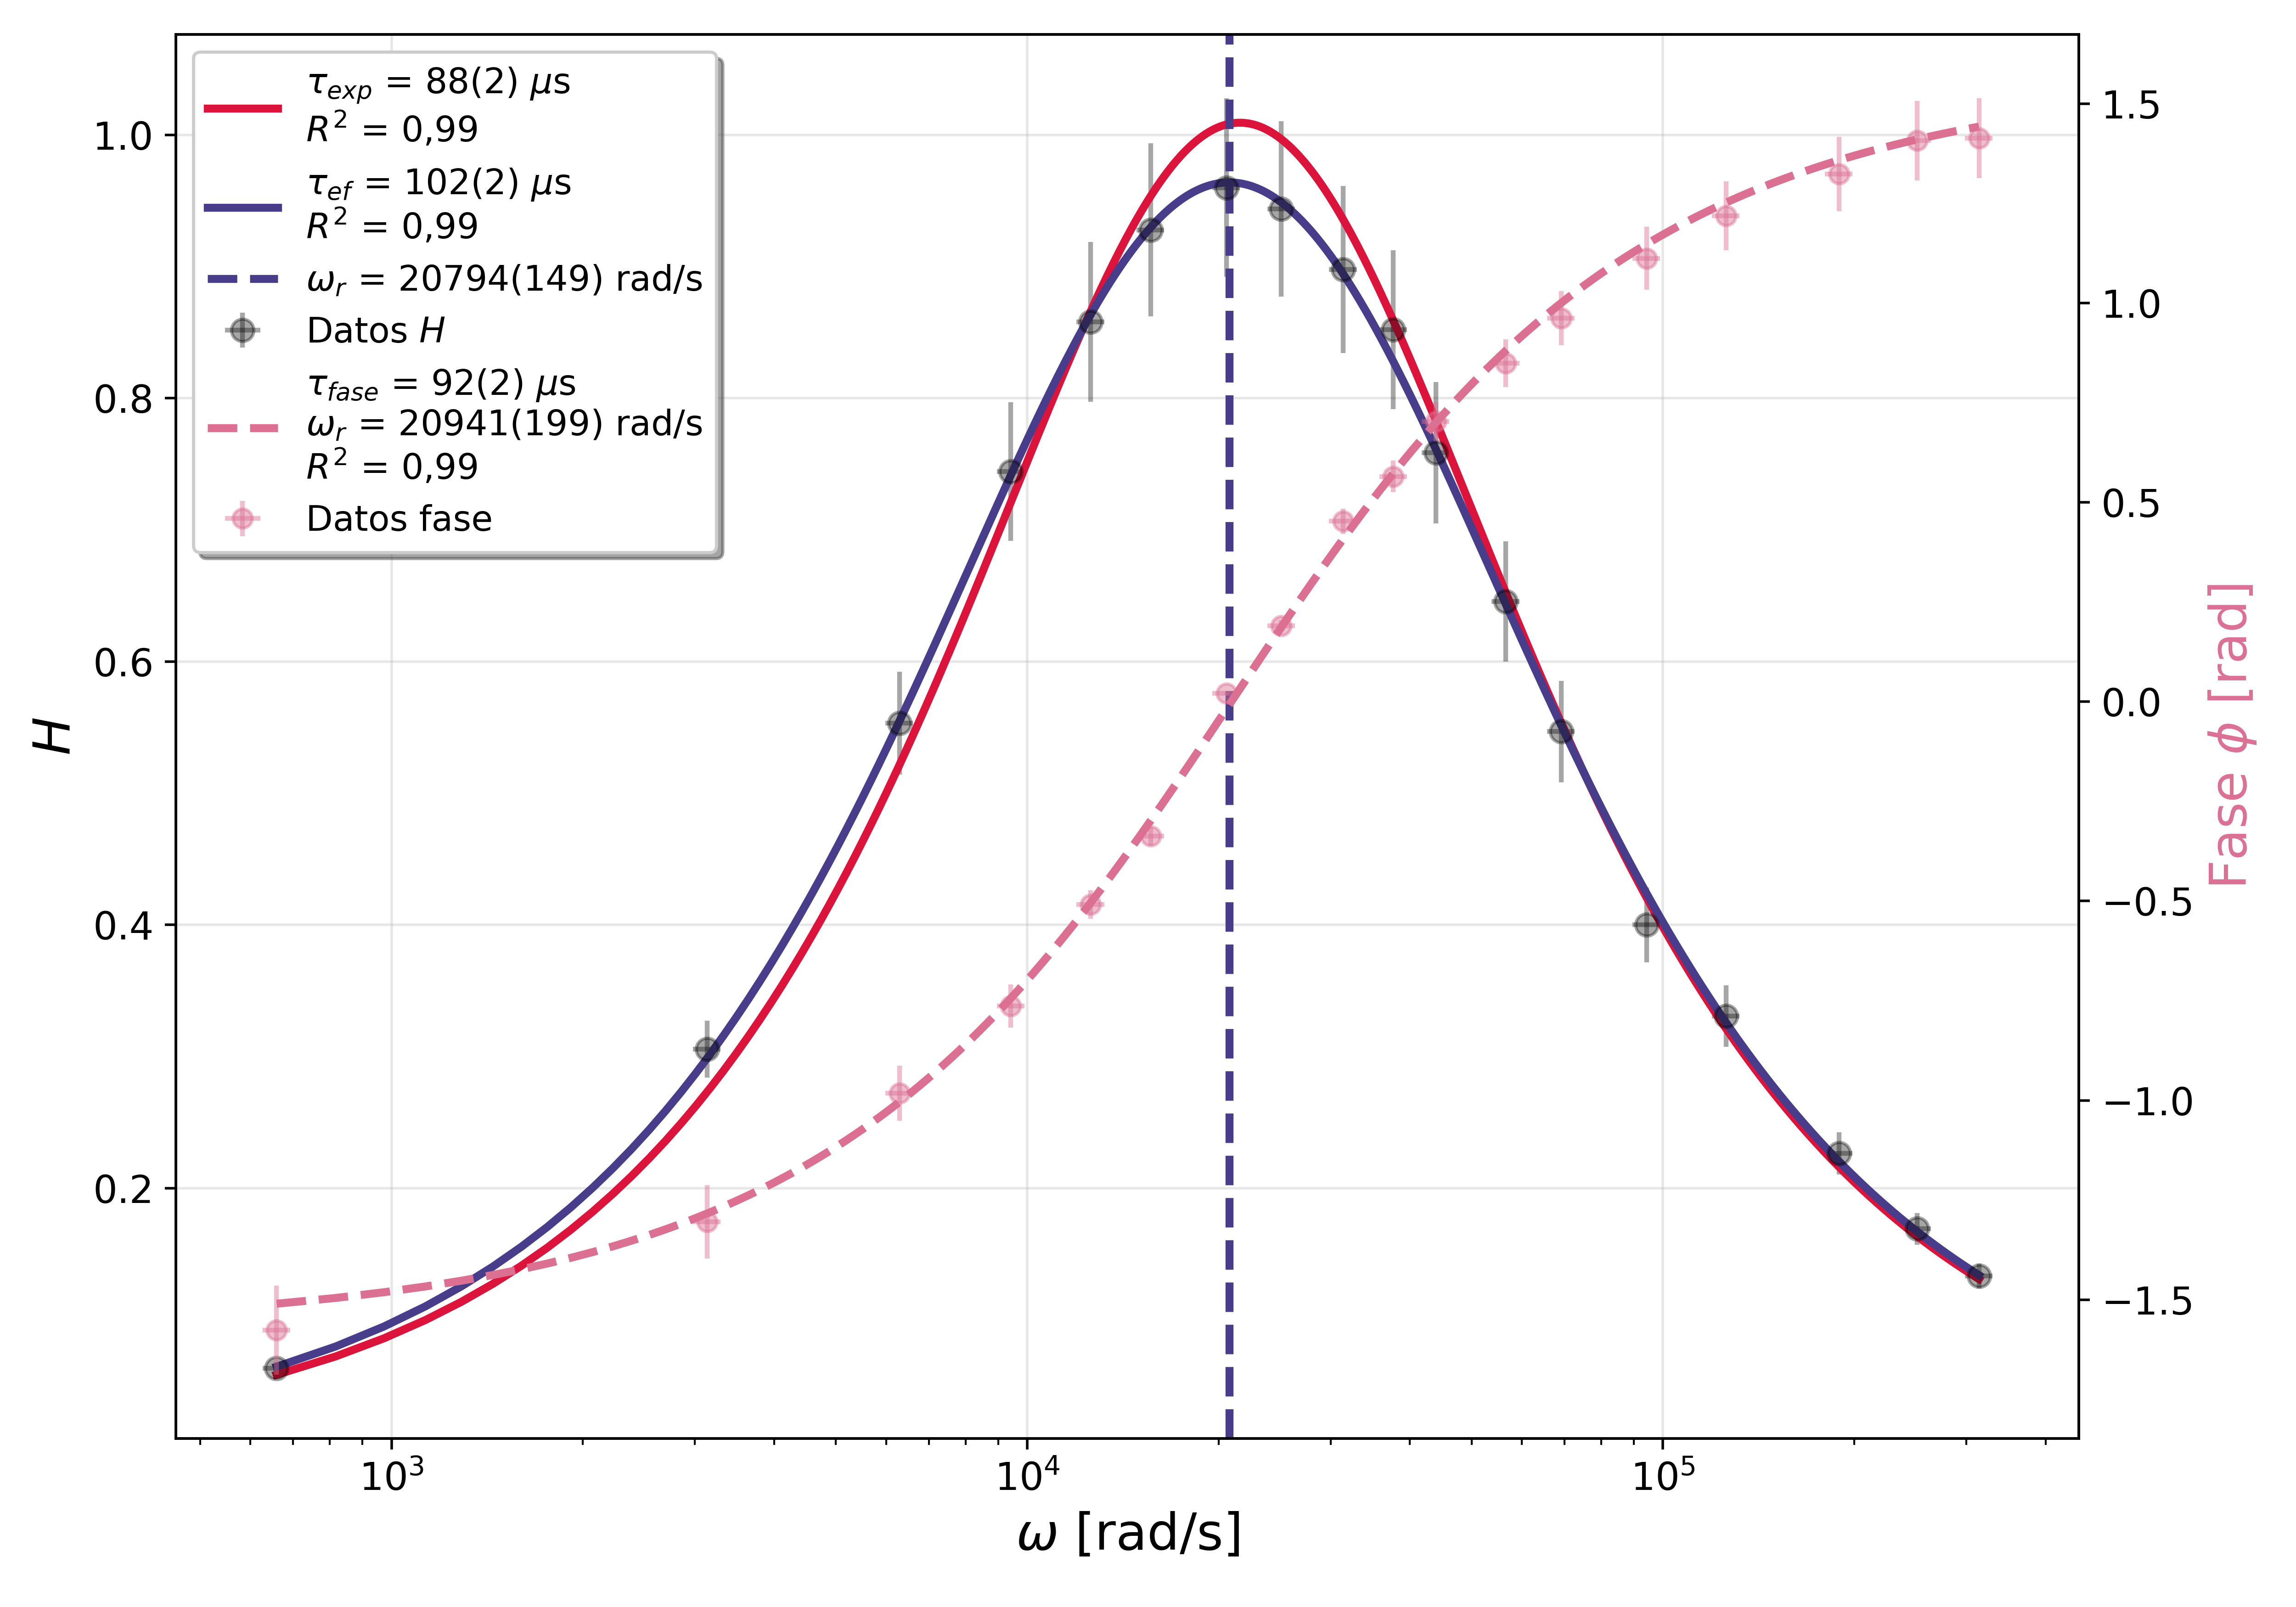
\includegraphics[width=0.7\linewidth]{gráficos/bode_completo_rlc.png}
    \caption{Ajustes realizados para la determinación de $\omega_r$, donde se indica en rojo el ajuste con $\tau_{exp}$ fijo. En azul, se presenta el ajuste con $\tau_{ef}$ como parámetro libre, junto a una línea vertical punteada del mismo color, la cual indica la posición de $\omega_r$. De igual forma, se presenta en rosa el ajuste realizado para el desfasaje, dejando a $\tau_{fase}$ como parámetro libre. Cerca de la línea azul punteada es posible observar como la curva correspondiente al ajuste de $\tau_{exp}$ se aleja de los datos experimentales.}
    \label{fig:tau_RLC}
\end{figure}
En el ajuste realizado para \(\tau\) libre se obtuvo \(\tau_{ef}\) = 102(2) \SI{}{\micro\second}, que presenta discrepancias con el valor \(\tau_{exp}\) = 88(2) \SI{}{\micro\second} obtenido para el circuito \(RC\). A su vez, es notorio en los gráficos de los ajustes que ambos métodos son compatibles lejos de la frecuencia de resonancia, pero difieren al acercarse a la misma. Esto se debe a que en la frecuencia de resonancia el inductor y el capacitor dejan de interferir en el circuito, actuando como un cable el cual no es ideal. Esto agrega una resistencia \(R_L\) la cual se asocia al inductor en el circuito, por lo que utilizando el valor nominal de la resistencia, denotando que \(R_{ef}=R + R_L\), fue posible cuantificar el valor de resistencia agregado por el inductor siendo de $R_{L}$ = \SI{157(9)}{\ohm}. El valor de la inductancia desconocida se obtuvo a partir del ajuste con $\tau_{ef}$, obteniendo $L$ = 2,6(2) \(\times 10^{-2}\) \SI{}{\henry}.

Se realizó el diagrama de Nyquist para el circuito RLC, presentado en la \autoref{fig:nyquist_RLC}, correspondiente a la medición realizada sobre la resistencia. Se presenta la serie de datos experimentales superpuesta a su curva teórica, dada por la ecuación \eqref{eq:moduloRLC} junto a su fase asociada \eqref{eq:desfasajeRLC}, la cual resulta compatible con el diagrama de Nyquist esperado para un circuito RLC. 

\begin{figure}[H]
    \centering
    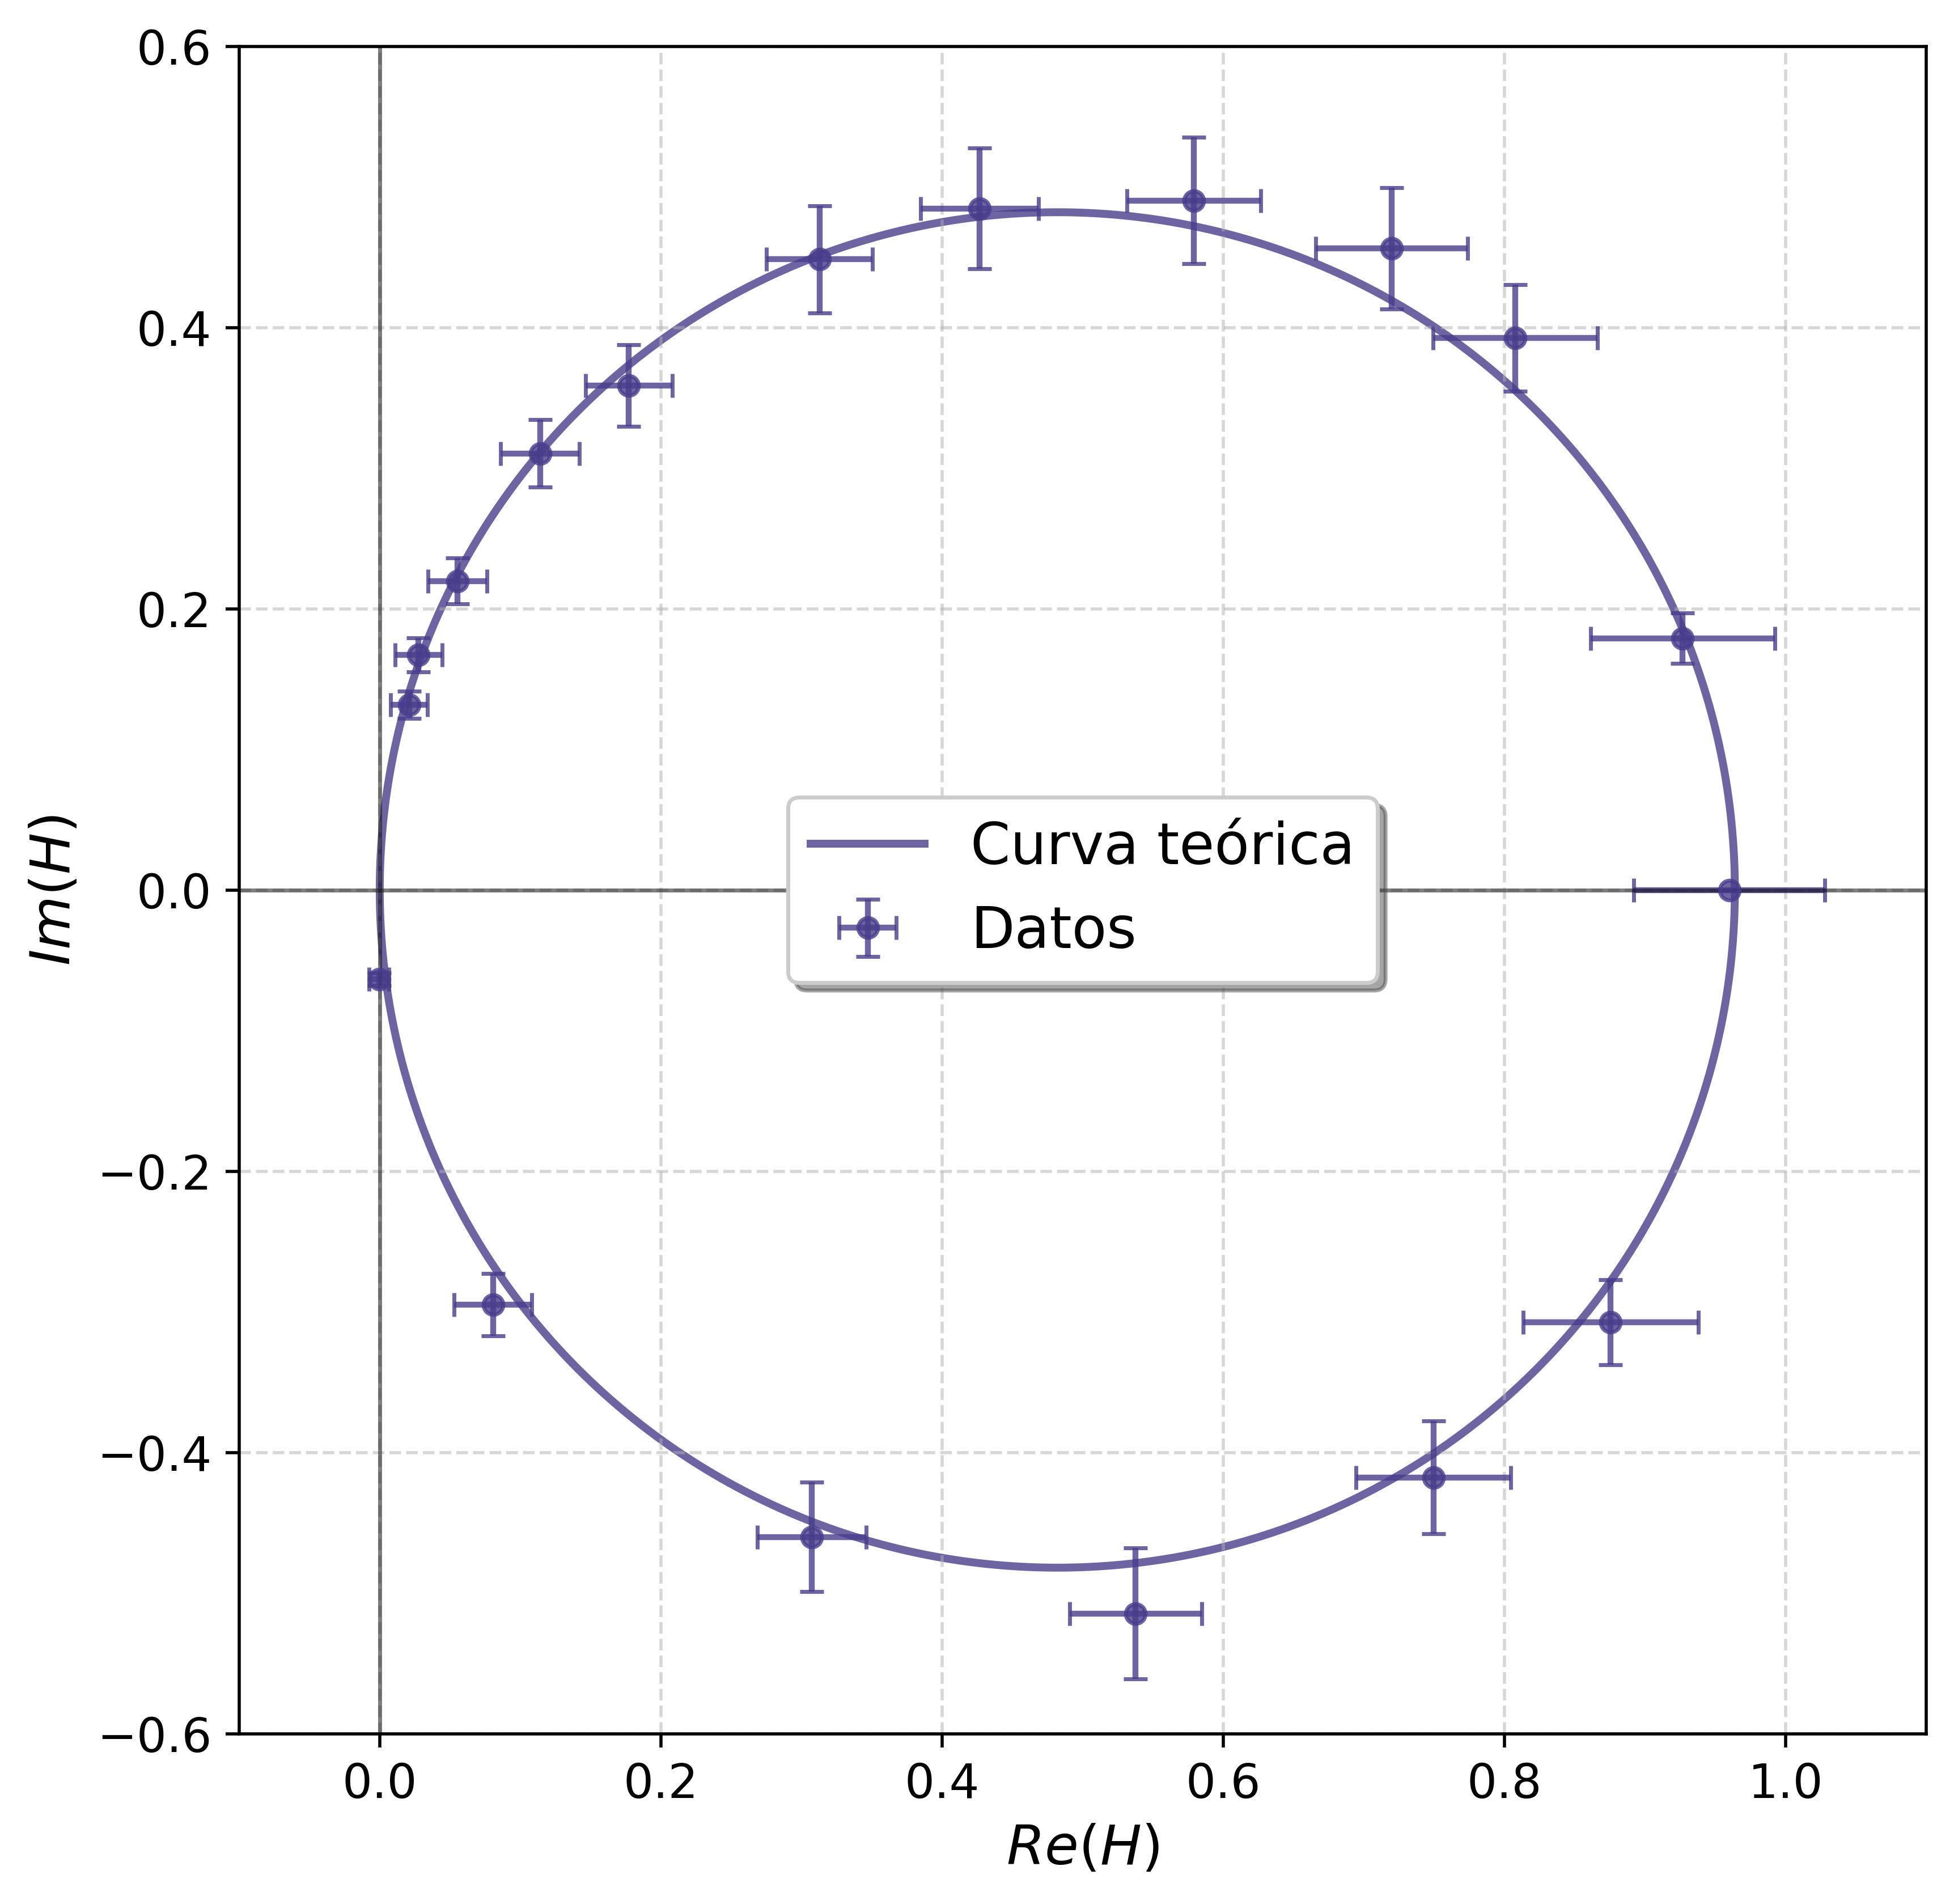
\includegraphics[width=0.5\linewidth]{gráficos/nyquist_RLC_teoria.png}
    \caption{Diagrama de Nyquist realizado para los datos obtenidos con el circuito RLC, junto a su curva teórica correspondiente.}
    \label{fig:nyquist_RLC}
\end{figure}

